\chapter{Wyznaczanie średnicy}
% wstęp do problemu
% Jednym z zagadnień, w którym kluczowym jest wyznaczanie średnicy
% zbioru punktów jest problem klastrowania. Klastrowanie zbioru to
% grupowanie jego elementów o podobnych właściwościach. Można zauważyć,
% że elementy klastra o mniejszej średnicy są ze sobą ściślej powiązane
% niż w klastrze dużym. Przez wielkość klastra mamy na myśli jego
% \emph{rozrzucenie}, czyli największą odległość między dwoma punktami
% klastra. Jeśli mamy więc zbiór punktów podzielić na $K$ klastrów,
% pożądany jest taki podział aby największa średnica klastra była
% możliwie mała. % przeredagować

% definicja
Problem ogólny średnicy dowolnego zbioru można przedstawić
następująco: jeśli danych jest $N$ punktów na płaszczyźnie, znaleźć
dwa punkty najbardziej odległe od siebie. Problem można rozwiązać
metodą naiwną wyznaczając odległość wszystkich $N(N-1)/2$ par punktów
i wybierając największą z nich. Jednak nawet dlat tak elementarnych
operacji możemy szukać bardziej efektywnych rozwiązań.

% Wiemy, że istnieje algorytm o złożoności $O(n\log{n})$,
% przekształcając problem rozłączności zbiorów w problem średnicy [1].
% Warto więc zastanowić się czy właściwości wielokąta wypukłego pomogłby
% nam uzyskać lepszy algorytm dla uzyskania średnicy zbioru. Skorzystamy
% z następującego twiedzenia:

% % nawiązać do spostrzeżenia, że problem 'średnica zbioru' zawiera się
% % w/lub równa 'srednica wielokąta wypukłego'

% \begin{twierdzenie}[Hocking-Young 1961]
%   Średnica zbioru jest równa średnicy jego otoczki wypukłej.
% \end{twierdzenie}

% W przypadku rozważań problemu na płaszczyźnie otoczka wypukła jest
% wielokątem wypukłym, możemy zdefiniować problem:

Dla wielokąta wypukłego zdefiniujmy problem:

\begin{problem}[Średnica wielokąta wypukłego]
  Jeśli dany jest wielokąt wypukły, znaleźć jego średnicę.
\end{problem}

Kluczowym dla algorytmu korzystającego z wypukłości wielokąta przy
wyznaczaniu średnicy jest następujące twierdzenie:

\begin{twierdzenie}[Yaglom-Bolyanskii 1961]
\label{thm:yagbol}
  Średnica figury wypukłej jest największa odległością między parą
  równoległych prostych wspierających.
\end{twierdzenie}

% idea algorytmu
Proste wspierające nie mogą przechodzić przez każdą parę punktów. Na
przykład żadne proste wpierające przechodzące przez $p_1$ i $p_5$
wielokąta z rysunku~\ref{fig:antipodal} nie mogą być równoległe, więc
$p_{1}p_{5}$ nie jest średnicą. Para punktów, przez które mogą
przechodzić proste wspierające jest nazywana punktami
\emph{antypodycznymi}. Z twierdzenia~\ref{thm:yagbol} wynika, że nie
musimy badać wszystkich par punktów, a jedynie pary antypodyczne,
szukając średnicy.

\begin{figure}[htp]
\label{fig:antipodal}
\centering
  \begin{tikzpicture}[scale=0.8]
    \convex
  \end{tikzpicture}
  \caption{}
\end{figure}

Przedstawiony zostanie teraz sposób znajdowania par punktów
antypodycznych. Rozważmy wielokąt przedstawiony na
rysunku~\ref{fig:antipodal}. Wybieramy dowolny wierzchołek $p_i$ i
przechodzimy w kierunku przeciwnym do ruchu wskazówek zegara po po
brzegu wielokąta tak długo, aż dojdziemy do wierzchołka $q_r$, który
jest najdalej pd $p_{i}p_{i-1}$. W taki sam sposób wyznaczamy
wierzchołek $q_l$ jako najdalszy od $p_{i}p_{i+1}$ przechodząc po
brzegu wielokąta zgodnie z ruchem wskazówek zegara. Łańcuch
wierzchołków od $q_r$ do $q_l$, z nimi samymi włącznie tworzy zbiór
wierzchołków, z których każdy tworzy parę antypodyczną z $p_i$. Możemy
zauważyć, że $p_{i},p_{r}$ jest parą antypodyczną wyłącznie wtedy gdy
istnieje prosta przecinająca $\angle \alpha_i$ i $\angle \alpha_s$
(rys.~\ref{fig:diameter}). Ze względu na to, że $C(p_i)$ jest
łańcuchem wypukłym, każdy wierzchołek $p_s$ należący do $C(p_i)$ jest
antypodyczny do $p_i$, a żaden wierzchołek nienależący do $C(p_i)$ nie
jest.  Obserwacja tego faktu umożliwia podanie algorytmu,
pozwalającego uzyskać wszystkie pary antypodyczne.

\begin{figure}[htp]
\label{fig:diameter}
  \centering
  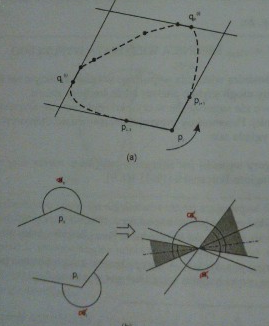
\includegraphics[width=0.3\textwidth]{img/diameter}
  \caption{[Rysunek roboczy]}
\end{figure}

% działanie algorytmu
Wejściem dla algorytmu jest wielokąt zadany jako lista wierzchołków ze
wskaźnikiem na swój następnik. Do określenia, który punkt leży
najdalej od odcinka $p_{0}p_{i+1}$ korzystamy funkcji ,,pola ze
znakiem trójkąta'' $p_{0}p_{i+1}p$, którą przedstawiono w
rozdziale~\ref{chap:pojecia} do wyznaczenia skrętności kąta, w
algorytmie oznaczonej jako $P$. W pierwszej części algorytmu w pętli
\textbf{while} szukamy pierszego najdalszego wierzchołka i oznaczamy
go jako $q_0$ (wiersze 4--6). Następnie będziemy wyznaczać łańcuch
$C(p_i)$, używając wskaźników $p$ i $q$ poruszających się w kierunku
odwrotnym do ruchu wskazówek zegara zaczynając odpowiednio od $p_0$ i
$q_0$ do momentu aż wskaźnik $q$ wróci do pozycji $p_0$ (wiersze
7--14). Po tym kroku zostaną wypisane wszystkie pary
antypodyczne. Znalezienie wierzchołka $q_0$ zajmuje w pesymistycznym
przypadku $N-1$ kroków, natomiast przejście po łańuchach $p_{0}q_{0}$
i $q_{0}p_{0}$ łącznie $N$ kroków. Specjalną sytuacją jest przypadek
gdy dwie krawędzie są równoległe (wtedy pole ze znakiem trójkąta
będzie równe dla dwóch wierzchołków tworzących krawędź równoległą),
która wymaga od nas dodatkowego kroku przy każdym wierzchołku (wiersze
15--19).

Krawędzi równoległych jest co najwyżej $N/2$, więc łącznie
algorytm nie wykonuje więcej niż $3N$ kroków. Mamy więc do czynienia
ze złożonością czasową $O(n)$.
% uzasadnienie działania
Algorytm wyszukując punkt antypodyczny dla punktu $p_{i+1}$ korzysta z
faktu, że nie może być on bliższy niż wierzchołek, który jest najdalej
od $p_i$. Związane jest to z wypukłością wielokąta --- dla dowolnego
wierzchołka $p$ można wyznaczyć taki wierchołek $q$, że odległość
kolejnych wierzchołków od $p$ do $q$ jest nierosnąca, zaś od $q$ do
$p$ niemalejąca.

\begin{figure}[htp]
\label{alg:antipodal}
\begin{algorithmic}[1]
\Procedure{Antipodal Pairs}{}

\State $p \gets p_N$
\State $q \gets NEXT[p]$

\While {$P(p, NEXT[p], NEXT[q]) > P(p,NEXT[p],q)$}
    \State $q \gets NEXT[p]$
    \State $q_0 \gets q$

    \While {$q \neq p_0$}
        \State $print (p, q)$

        \While {$P(p, NEXT[p], NEXT[q] > P(p, NEXT[p], q))$}
            \State $q \gets NEXT[q]$

            \If {$(p, q) \neq (q_0,p_0)$}
                \State $print (p, q)$
            \EndIf
        \EndWhile

        \If {$P(p, NEXT[p], NEXT[q] = P(p, NEXT[p], q))$}
            \If {$(p, q) \neq (q_0, p_n)$}
                \State $print (p, NEXT[q])$
            \EndIf
        \EndIf
    \EndWhile
\EndWhile
\EndProcedure

\end{algorithmic}
\end{figure}

%%% Local Variables:
%%% mode: latex
%%% TeX-master: "masterthesis"
%%% TeX-engine: xetex
%%% End:
